O hardware utilizado aqui será o  TIVA \texttrademark ~~ TM4C1294NCPDT, um kit de desenvolvimento da empresa Texas Instruments que possui um microcontrolador baseado no processador ARM Cortex-M4. A tabela \ref{tab:CaracteristicasMicro} traz suas principais características.

%% TABELA DE CARACTERISTICAS BASICAS %%%%%%%%%%

% \begin{table}[!h]
% \centering

\begin{longtable}{|l|l|}

\hline
\cellcolor[HTML]{343434} \color[HTML]{FFFFFF} Características & \cellcolor[HTML]{343434} \color[HTML]{FFFFFF} Descrição \\
\hline
Núcleo & ARM Cortex-M4F\\
\hline
Performance & Operação até 120-MHz; 150 DMIPS \\
& (Dhrystone MIPS) de performance \\
\hline
Memória Flash & 1024 KB  \\
\hline
SRAM & 256 KB single-cycle System SRAM \\
\hline
EEPROM & 6KB  \\
\hline
ROM & ROM interna carregada com biblioteca  \\
 & TivaWare™  C Series \\
\hline
Interface de Periféricos Externos (EPI)  & Interface dedicada de 8-/16-/32-   \\ 
 &  bits dedicados a periféricos e memoria\\
\hline
 Verificação de Redundância & Função Hash de 16-/32- bits,  que suporta  \\
  Cíclica (CRC)   & quatro formas de CRC \\
\hline
\begin{comment}
 Função de Adulteração & Suporte para quatro entradas de  \\
 & adulteração e resposta de evento de  \\
 & adulteração configurável configurável  \\
\hline
\end{comment}
Universal Asynchronous  & 8 módulos UARTs \\
Receivers/Transmitter (UART) & \\
\hline
Quad Synchronous Serial & Quatro módulos de SSI com Bi- , Quad-\\
Interface (QSSI) &  e suporte avançado de SSI\\
\hline
Inter-Integrated Circuit ($I^{2}C$) & 10 módulos $I^{2}C$ com 4 velocidades \\
 & de transmissão\\
\hline
Controller Area Network (CAN) & 2 controladores CAN 2.0 A/B \\
\hline
Ethernet MAC & 10/100 Ethernet MAC \\
\hline
Ethernet PHY & PHY com IEEE 1588 PTP \\
\hline
Universal Serial Bus (USB) & USB 2.0 OTG/Host/Device  \\ 
& com ULPI interface e suporte a Link   \\
& Power Management (LPM) \\
\hline
Micro Acesso Direto à Memória ($\mu DMA$) & Controlador ARM$\copyright$ PrimeCell$\copyright$  \\
& 32-channel configurável  $\mu DMA$ \\
\hline
General-Purpose Timer (GPTM) & 8 blocos 16/32-bit GPTM \\
\hline
Watchdog Timer (WDT) & 2 Watchdog Timers \\
\hline
Hibernation Module (HIB) & Low-power battery-backed \\
 & Hibernation module \\
\hline
General-Purpose Input/Output (GPIO) & 15 physical GPIO blocks \\
\hline
Pulse Width Modulator (PWM) & 1 modulo PWM , com 4 geradores PWM  \\
 & e um  registador de controle,\\
 &  com um total de 8  saídas PWM.\\
\hline
Quadrature Encoder Interface (QEI) & Um modulo QEI \\
\hline
Analog-to-Digital Converter (ADC) & 2 modulos ADC de 12-bit\\
 & taxa de 2 milhões de amostras/segundo\\
\hline
Controlador Comparador Analógico & Três comparadores analógicos \\
& independentes \\
\hline
Comparador Digital & 16 comparadores digitais \\
\hline
JTAG e Serial Wire Debug (SWD) & 1 modulo JTAG  com ARM SWD\\
& integrado \\
\hline
Encapsulamento & 128-pin TQFP \\
\hline
Temperatura de Operação & $-40 \degree C$ até $105 \degree C$ \\
\hline
\caption{Características Básicas - TM4C1294NCPDT \cite{DATASHEET_TIVA}}
\label{tab:CaracteristicasMicro}
\end{longtable}
% \end{table}

%%%%%%%%%%%%%%%%%%%%%%%%%%%%%%%%%%%%%%%%%%%%%%%%%%%%%%%


O TM4C1294NCPDT possui dois barramentos. Um desses é responsável pela conexão padrão entre o núcleo de processamento e os periféricos, o \emph{Advanced Peripheral Bus} (APB). Já o outro, o \emph{Advanced High-Performance Bus} (AHB), é um barramento especial que pode ser requisitado da maioria dos periféricos e, possui uma resposta muito mais rápida por ser exclusivo. O esquema dos barramentos é mostrado no diagrama de blocos da figura \ref{fig:DiagramaBlocosTiva}.


\begin{figure}[H]
\centering
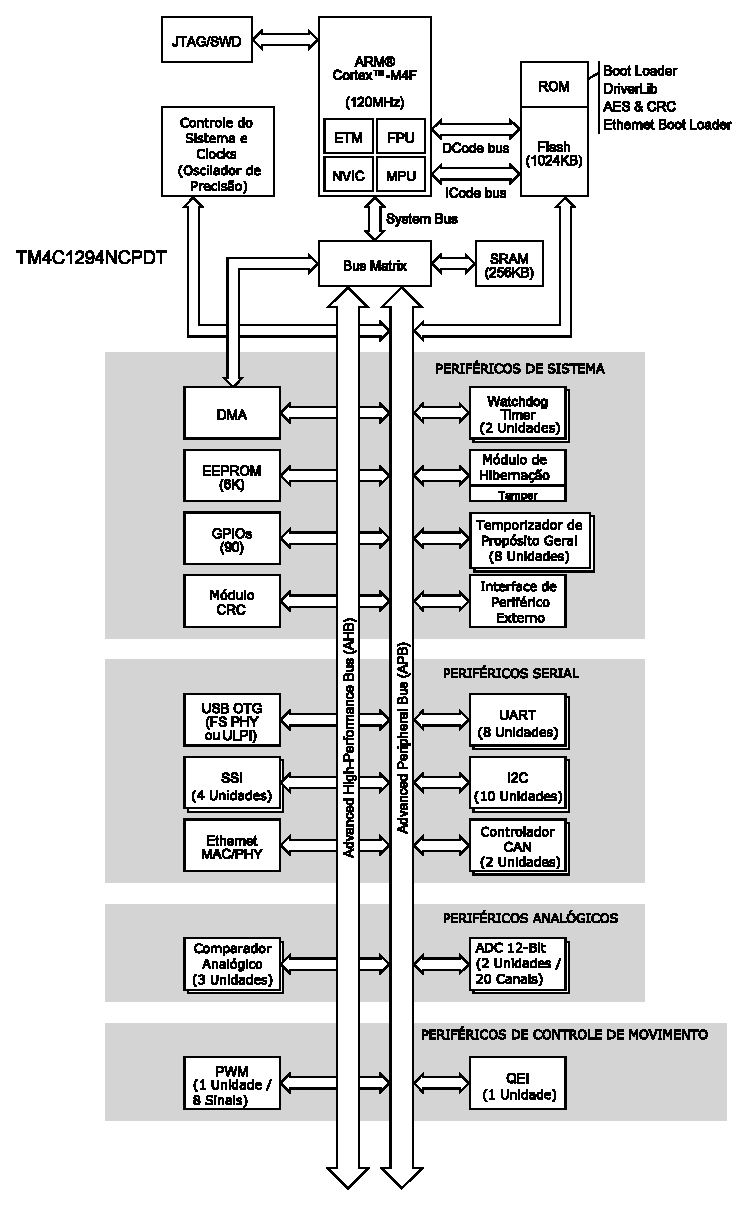
\includegraphics[width=0.8\textwidth] {DiagramaBlocosTiva.eps}
    \caption{Diagrama de Blocos - TM4C1294NCPDT \cite{DATASHEET_TIVA}}
    \label{fig:DiagramaBlocosTiva}
\end{figure}

%%%%%%%%%%%%%%%%%%%%%%%%%%%%%%%%%%%%%%%%%%%%%%%%%%%%%%%